\documentclass{../latex/utmreport}
\newcommand{\ReportTitle}{Lab 1: The OS as a Resource Manager}
% Shared title-page and PDF metadata for every laboratory report.
\newcommand{\StudentName}{Gafenco Victor}
\newcommand{\StudentGroup}{FAF-241}
\newcommand{\CourseName}{Operating Systems}
\newcommand{\InstructorName}{Patricia Reitman}
\newcommand{\InstructorTitle}{Assistant lecturer}
\newcommand{\ReportCity}{Chișinău}
\newcommand{\ReportYear}{2026}
\newcommand{\CourseRepository}{https://github.com/yoda-dinmd/os-labs}

\selectlanguage{english}
\utmlogo{../latex/assets/UTM_Logo_English.jpeg}
\institution{Technical University of Moldova}
\faculty{Faculty of Computers, Informatics, and Microelectronics}
\department{Department of Software Engineering}
\studyprogramme{Software Engineering Study Programme}
\documenttype{Laboratory report}
\student{\StudentName}{\StudentGroup}
\supervisor{\InstructorName}{\InstructorTitle}
\renewcommand{\UTMCoordinatorLabel}{Instructor}
\cityyear{\ReportCity}{\ReportYear}
\reportsubtitle{\CourseName}
\hypersetup{pdfauthor={\StudentName},pdfsubject={\CourseName},
  pdftitle={\ReportTitle}}
\reporttitle{\ReportTitle}
\addto\captionsenglish{\renewcommand{\figurename}{Figure}\renewcommand{\tablename}{Table}\renewcommand{\bibname}{References}}
\renewcommand{\figurename}{Figure}
\renewcommand{\tablename}{Table}
\renewcommand{\bibname}{References}
\usepackage{float}
\usepackage{placeins}
\setlength{\emergencystretch}{2em}
\newcommand{\code}[1]{\texttt{\detokenize{#1}}}
% Keep screenshots beside their observations, with bounded height and width.
\newcommand{\screenshot}[4][\textwidth]{%
  \begin{figure}[H]
    \centering
    \includegraphics[width=#1,height=0.62\textheight,keepaspectratio]{screenshots/#2}
    \caption{#3}\label{#4}
  \end{figure}}
\newcommand{\reportreferences}[2]{%
  \clearpage\phantomsection\addcontentsline{toc}{chapter}{References}
  \begin{thebibliography}{9}
    \bibitem{handout} Technical University of Moldova, FCIM / FAF.
    \textit{#1}. Operating Systems laboratory handout, academic year 2026--2027.
    Supplied course document: \code{#2}.
  \end{thebibliography}}


\begin{document}
\makeutmreporttitlepage
\tableofcontents
\clearpage

\begin{utmabstract}[Abstract]
This laboratory examines how an operating system manages files, processes,
memory, and devices using an Ubuntu virtual machine. Terminal commands were
used to create and remove files, change access permissions, inspect running
processes, terminate a background task, and read kernel information through
the process filesystem. Memory and storage commands provided quantitative
snapshots of the machine. The file owner and group were both \code{victor};
the process listing contained approximately 222 processes; memory inspection
reported 3.3 GiB of total memory and no configured swap. The root filesystem
was mounted from \code{/dev/sda2} using ext4. Screenshots document each
resource-management task. Values from different captures are treated as
separate observations because resource usage changes during execution.
\utmkeywords{file permissions, processes, memory, devices, storage, linux}
\end{utmabstract}

\chapter*{Abbreviations}
\addcontentsline{toc}{chapter}{Abbreviations}
\noindent\begin{tabularx}{\textwidth}{lY}
OS & operating system \\
VM & virtual machine \\
PID & process identifier \\
RAM & random-access memory \\
RSS & resident set size \\
I/O & input/output \\
GiB, MiB, KiB & binary units: $2^{30}$, $2^{20}$, and $2^{10}$ bytes \\
\end{tabularx}

\utmintroduction
The operating system mediates between programs and hardware by allocating
resources and enforcing access rules. This laboratory follows the four
resource-management areas in the course handout: files, processes, memory,
and devices~\cite{handout}. The work was performed through the terminal in an
Ubuntu VM. Figures throughout the report are the student's captured outputs.

The VM uses account \code{victor}, hostname \code{oscourse}, and the
\code{7.0.0-34-generic} Linux kernel on x86-64. The initial capture shows seven
minutes of uptime. The work directory was \path{/home/victor/os-lab1}.
The screenshot below records the environment. Later measurements were
taken in separate sessions and should not be interpreted as simultaneous.
\begin{figure}[H]
\centering
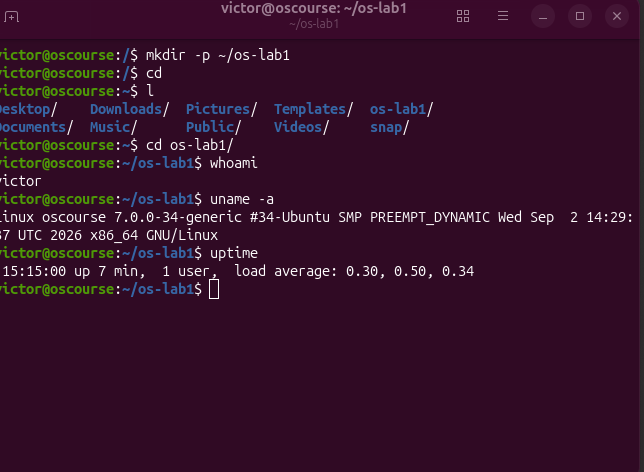
\includegraphics[width=\textwidth,height=0.62\textheight,keepaspectratio]{screenshots/L1_01_environment.png}
\end{figure}

\chapter{File and directory management}
The filesystem presents data as a hierarchy of named objects. This part
examined directory contents, basic file operations, ownership, and access
permissions.

\section{Directory structure}
The home directory contains personal files and application settings. The
\code{/etc} listing includes configuration entries such as
\code{NetworkManager}, \code{X11}, and \code{adduser.conf}.
Figure~\ref{fig:directories} shows these listings.

Two directories directly under the root are \code{/etc}, which contains
system configuration, and \code{/home}, which contains users' home
directories. The captured directory commands show the home and
\code{/etc} contents; a direct listing of \code{/} was not captured.
\screenshot{L1_02_directories.png}{Working, home, and configuration directory listings}{fig:directories}

\section{Creation, copying, renaming, and removal}
The command \code{echo} created \code{note.txt} containing
\code{hello operating systems}. Copying it produced \code{copy.txt}, which
was renamed to \code{renamed.txt}. Both files were 24 bytes long.
After \code{rm renamed.txt}, the directory contained only \code{note.txt}.
Figure~\ref{fig:files} documents the commands and the before-and-after
listings. The owner and group of both created files were \code{victor}.
\screenshot{L1_03_files.png}{Creating, copying, renaming, and deleting a file}{fig:files}

\section{Ownership and permissions}
The initial mode was \code{-rw-rw-r--}. After
\code{chmod 600 note.txt}, it became \code{-rw-------}. In this ten-character
field, the first character identifies a regular file. The next three characters
give the owner read and write permission without execute permission. The
remaining groups of three give the group and other users no access.
The command \code{chmod 644 note.txt} restored \code{-rw-r--r--}, allowing
other users to read while retaining write permission only for the owner.
Figure~\ref{fig:permissions} shows all three modes.
\screenshot{L1_04_permissions.png}{Permission changes from the initial mode to 600 and 644}{fig:permissions}

\chapter{Process management}
A process is an executing program with an identifier and execution state.
Process-listing tools and the kernel's \code{/proc} interface expose the
tasks being managed by the OS.

\section{Listing processes and identifying PID 1}
The initial \code{ps aux | wc -l} command printed 223, including the output
header. The header-free command \code{ps -e --no-headers | wc -l} printed
222. This indicates approximately 222 processes at that snapshot; counts can
change even between consecutive commands.

Process 1 was \code{systemd}, running as root from
\code{/usr/lib/systemd/systemd}. It is the initial userspace process and
manages system services. Figure~\ref{fig:processes} records its identity and
the process counts.
\screenshot{L1_05_processes.png}{Process listing, approximate count, and identity of PID 1}{fig:processes}

The live monitor in Figure~\ref{fig:top} showed 251 tasks: one running and
250 sleeping, with no stopped or zombie tasks. This later snapshot differs
from the earlier \code{ps} count because the VM's workload changed.
\screenshot{L1_06_top.png}{Live CPU, memory, and process information from top}{fig:top}

\section{Starting and terminating a background task}
The command \code{sleep 300 &} started a background process with PID 9453.
The shell's \code{jobs} command and the system-wide \code{ps} listing both
showed it running. After \code{kill "$PID"}, the shell reported termination.
The final process lookup printed only a header, indicating that the process
was no longer present. Figure~\ref{fig:background} records this lifecycle.
\screenshot{L1_07_background.png}{Starting, finding, and terminating a background process}{fig:background}

\section{Inspecting process state through the kernel}
A separate \code{sleep} process had PID 9765. Its directory under
\code{/proc} contained entries such as \code{cmdline}, \code{fd},
\code{maps}, and \code{status}. The status file reported
\code{State: S (sleeping)}. This is interruptible sleep: the process waits
rather than actively executing on the CPU. Figure~\ref{fig:proc} also shows
the process and parent identifiers and its termination after inspection.
\screenshot{L1_08_proc.png}{Kernel-exposed status of the sleeping process}{fig:proc}

\chapter{Memory management}
The OS distributes physical memory between processes and uses reclaimable
cache to improve performance. System totals and per-process memory fields
provide different views of this allocation.

\section{Physical memory and swap}
Table~\ref{tab:memory} summarizes the \code{free -h} snapshot.
\begin{table}[H]
\caption{Observed memory totals}\label{tab:memory}
\centering
\begin{tabularx}{0.8\textwidth}{|Y|l|}\hline
\textbf{Field} & \textbf{Reported value}\\\hline
Total RAM & 3.3 GiB\\\hline
Used RAM & 2.4 GiB\\\hline
Free RAM & 272 MiB\\\hline
Available RAM & 962 MiB\\\hline
Configured swap & 0 B\\\hline
\end{tabularx}
\end{table}
Free memory is unused memory, whereas available memory also accounts for
memory that can be reclaimed for applications. Swap is backing space used
to move eligible memory pages out of RAM; none was configured in this
capture. The subsequent \code{/proc/meminfo} reading reported
\code{MemTotal: 3479664 kB}. The commands were separate snapshots, so their
free and available values need not match exactly.

\section{Resident memory of a sleeping process}
The process with PID 9978 reported \code{VmRSS: 7752 kB}, approximately
7.57 MiB. This is more than the source-level simplicity of \code{sleep}
alone suggests, but an executing program still requires code, stack, runtime
data, and possibly shared library pages. RSS counts resident shared pages
as well as private pages and therefore does not measure exclusively owned
memory. Figure~\ref{fig:memory} records both system and process readings.
\screenshot{L1_09_memory.png}{System memory, swap, and resident memory of sleep}{fig:memory}

\chapter{Device and storage management}
Storage tools connect logical mount points with the devices that provide
their data. The device directory also exposes file-like interfaces for I/O.

\section{Root filesystem and disk usage}
The root filesystem \code{/} was mounted from \code{/dev/sda2}, using
ext4, as confirmed by \code{findmnt /}. The \code{df -h} output reported
49 GiB total, 7.5 GiB used, 39 GiB available, and 17\% utilization.
The block-device listing showed a 50 GiB virtual disk named \code{sda}.
The working folder occupied 12 KiB according to \code{du -sh}.
Figure~\ref{fig:storage} connects the disk, partition, and mount point.
\screenshot{L1_10_storage.png}{Mounted filesystems, block devices, and working-folder size}{fig:storage}

\section{Device entries and file-like interfaces}
The entry \code{/dev/cdrom} points to \code{sr0}, the VM's virtual optical
drive. The storage listing shows VirtualBox Guest Additions media mounted
from \code{/dev/sr0}. The entry \code{/dev/null} is a character device that
discards written data and returns end-of-file when read.

The UNIX expression ``everything is a file'' describes how many resources,
including devices, are exposed through operations such as opening, reading,
and writing. It does not mean every resource is a regular disk file.
Figure~\ref{fig:devices} shows device types, symbolic links, and mounts.
\screenshot{L1_11_devices.png}{Device entries and filesystem mount interfaces}{fig:devices}

\utmconclusions
The OS manages files and directories, whose ownership and permissions were
inspected with \code{ls -l}. It manages processes, visible with \code{ps},
and memory, visible with \code{free -h}. It also manages devices and storage,
which were inspected with \code{lsblk}.

The observations demonstrate permission enforcement, process termination,
kernel-exposed process state, and the association between a mounted
filesystem and its device. Process counts and memory use varied between
captures, as expected for a running system. All reported measurements are
taken from the supplied terminal screenshots.
\end{document}
